\section{РЕЗУЛЬТАТЫ РАБОТЫ}

\subsection{Характеристика условий и места применения разработки}

Web-справочник был специально разработан для использования медицинскими работниками скорой медицинской помощи в условиях их оперативной деятельности. Из-за особенностей этой области и ее требований, разработанный справочник обеспечивает оптимальную поддержку и удобство использования в рабочих условиях, связанных с оказанием скорой медицинской помощи. Он предоставляет удобный и мгновенный доступ к необходимой медицинской информации, что позволяет работникам быстро находить нужные данные и принимать информированные решения.

Web-справочник находит свое применение в следующих ситуациях:

\begin{itemize}
    \item Экстренные ситуации: в случаях, требующих немедленной реакции, медицинским работникам необходимо быстро получить доступ к актуальной информации о симптомах, диагнозах и процедурах оказания помощи. Web-справочник обеспечивает оперативный поиск и доступ к рекомендациям и протоколам, помогая медицинским работникам принимать правильные решения в экстренных ситуациях;
    \item Полевые условия: врачи и санитары, работающие на местах происшествий или в других условиях, где доступ к стационарным справочникам ограничен, могут полагаться на web-справочник для получения необходимой информации о болезнях;
    \item Обновление знаний: web-справочник предоставляет возможность медицинским работникам быть в курсе последних достижений в медицинской науке и практике. Для обновления знаний, материалы в справочнике могут быть обновлены администратором вручную. Таким образом, медицинские работники могут легко получать информацию из обновленных источников и оставаться информированными о последних достижениях в своей области.
\end{itemize}

Важными характеристиками использования разработанного web-справочника в работе медицинских работников скорой помощи являются:

\begin{itemize}
    \item Оптимизированный поиск информации: медицинским работникам скорой помощи часто требуется мгновенный доступ к конкретным медицинским справочным данным. Разработанный справочник обеспечивает быстрый и эффективный поиск по ключевым статьям, позволяя оперативно находить нужную информацию и принимать соответствующие решения;
    \item Удобное хранение данных: разработанный справочник хранит данные по категориям, что дает медицинским работникам скорой помощи быстрый доступ к наиболее важным и актуальным данным, если у них нет времени выполнять поиск;
    \item Обновляемая и достоверная информация: в медицинской практике необходимо иметь доступ к актуальным и проверенным справочным материалам. Разработанный справочник может обновляться и поддерживаться, обеспечивая медицинским работникам достоверную информацию, соответствующую последним стандартам и протоколам лечения;
    \item Возможность расширенного поиска: web-справочник также предоставляет удобную функцию перехода на посторонний сайт для дополнительного поиска информации. При использовании поисковой строки в справочнике, пользователю отображается опция "Поиск по справочнику MSD" с прикрепленной ссылкой. При клике на эту ссылку, пользователь может открыть страницу с результатами поиска по своему запросу на постороннем сайте в новой вкладке браузера. Таким образом, врачам не требуется открывать другой сайт или повторно вводить запрос, сохраняя все процессы поиска и получения информации в одном месте — в web-справочнике. Это обеспечивает удобство использования и экономит время медицинского персонала.
\end{itemize}

При тестировании web-справочника были проведены проверки, направленные на обеспечение корректности, надежности и эффективности приложения. Главной целью тестирования было проверить соответствие разработанного функционала заявленным требованиям.

Одним из аспектов, проверенных в ходе тестирования, было отображение и доступность информации в интерфейсе web-справочника. Важно было убедиться, что информация корректно отображается пользователю и соответствует заданному макету. Это позволяет обеспечить удобство использования приложения и удовлетворение потребностей пользователей.

Другим аспектом тестирования была проверка правильности функционирования различных модулей и компонентов приложения. В ходе тестирования проверялась правильность работы функции поиска по названию статьи. 

Результаты тестирования подтверждают соответствие разработанного приложения заявленным требованиям, данные функциональности работают корректно и обеспечивают надежность и эффективность его работы.

\subsection{Результаты работы разработанного программного кода}

В результате работы был создан web-справочник, который предоставляет пользователю следующие функциональности:

\begin{itemize}
    \item Интуитивно понятный интерфейс пользователя: интерфейс разработан с учетом простоты и интуитивности, чтобы пользователи могли быстро ориентироваться и находить нужную информацию. Он предоставляет удобную навигацию, плавные переходы между разделами, интуитивные иконки и элементы управления, а также четкую организацию контента, что можно увидеть на рисунке~\ref{fig:main-page};

\begin{figure}
  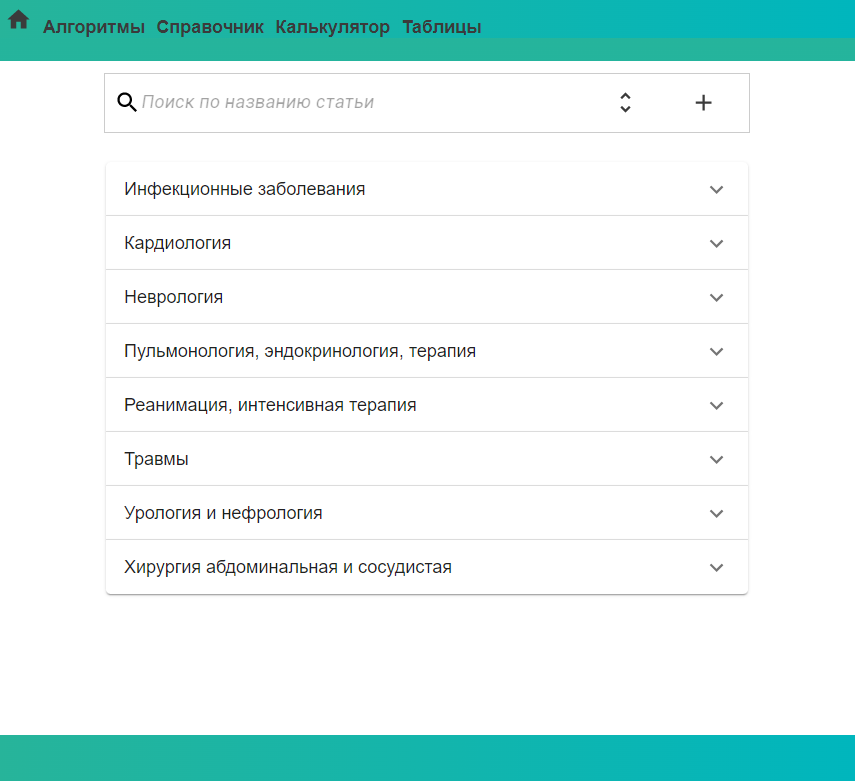
\includegraphics[scale=0.6]{styles/diploma/inc/ГлСтраница.png}
  \caption{Интерфейс справочника}
  \label{fig:main-page}
\end{figure}

    \item Поисковая строка: в справочнике реализована поисковая строка, представленная на рисунке~\ref{fig:search}, которая позволяет пользователям вводить ключевые слова и получать соответствующие результаты поиска. Механизм поиска анализирует запросы пользователей и находит наиболее релевантные статьи и информацию, соответствующую введенным ключевым словам;

\begin{figure}
  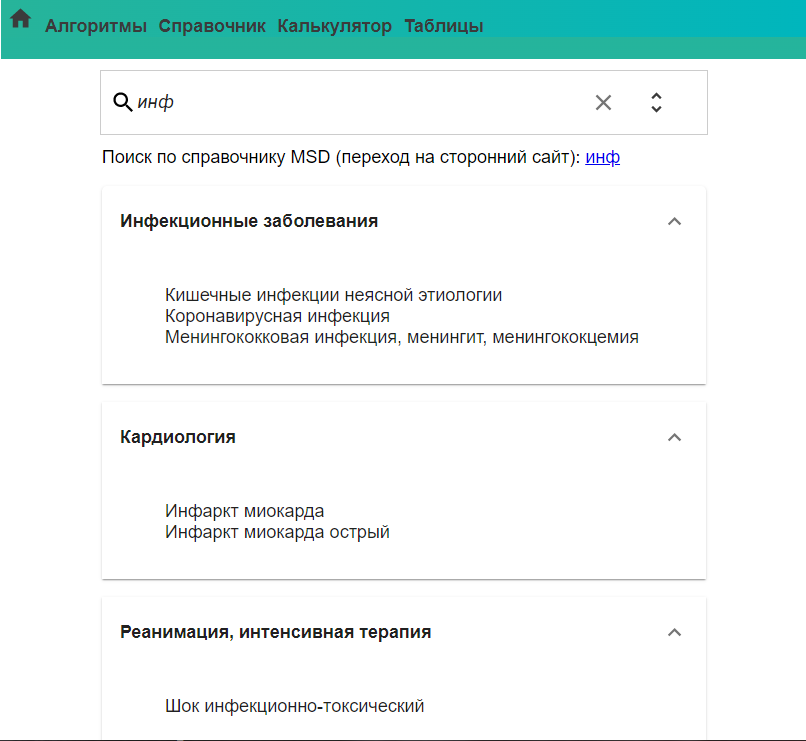
\includegraphics[scale=0.6]{styles/diploma/inc/Поиск.png}
  \caption{Поиск по справочнику}
  \label{fig:search}
\end{figure}

    \item Категории для классификации информации: справочник предоставляет организацию информации в виде категорий, что облегчает пользователю поиск нужных разделов. Пользователи могут выбирать соответствующую категорию и легко получать доступ к нужным статьям внутри этой категории;
    \item Отображение информации: разработанный справочник отображает информацию, содержащуюся в статье, соответствующим образом, согласно шаблону, указанному в предыдущих разделах. После выполнения поиска или выбора статьи пользователь может просмотреть кликнуть на статью. Если содержимое статьи есть в базе данных, открывается страница с текстом статьи, как на рисунке~\ref{fig:article}. В случае, если текст статьи не загружен в справочник, происходит переадресация на соответствующую страницу.

\begin{figure}
  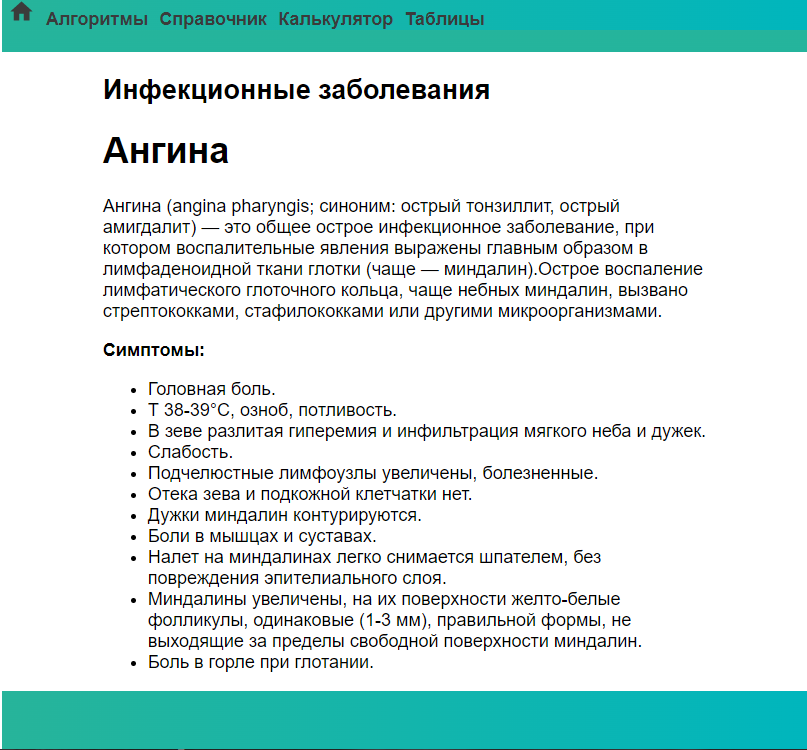
\includegraphics[scale=0.6]{styles/diploma/inc/Статья.png}
  \caption{Отображение статьи справочника}
  \label{fig:article}
\end{figure}

\end{itemize}

Таким образом, разработанный программный код обеспечивает удобство использования web-справочника, позволяя пользователям быстро находить и получать необходимую медицинскую информацию. Интуитивный интерфейс, функция поиска, категоризация информации и правильное отображение результатов работы являются ключевыми достижениями данного проекта. Получившееся приложение соответствует начальным требованиям.

\subsection{Технические характеристики разработанного решения и полученных результатов}

Разработанный web-справочник демонстрирует высокую производительность и надежность в процессе эксплуатации. Ниже приведены основные технические характеристики и результаты, достигнутые в процессе работы:

\begin{itemize}
    \item Производительность: время отклика на запросы пользователя осталось на приемлемом уровне даже при работе с большим объемом данных. Это позволяет пользователям быстро получать результаты поиска и просматривать информацию без задержек. Функция фильтрации и сортировки обеспечивает быстрое нахождение нужной информации, что улучшает пользовательский опыт;
    \item Надежность и стабильность: разработанное решение было тщательно протестировано и отлажено, чтобы обеспечить его надежную работу и минимизировать возможность ошибок или сбоев. Надежность системы особенно важна в контексте медицинской помощи, где быстрый и точный доступ к актуальной информации критически важен. Продолжительное использование и эксплуатация разработанного решения подтверждают его стабильность и надежность в реальных условиях.
\end{itemize}

Для дальнейшего развития и усовершенствования web-справочника можно рассмотреть следующие улучшения:

\begin{itemize}
    \item Расширение базы данных справочной информации и ее регулярное обновление обеспечат актуальность и полноту данных. Это может включать добавление новых статей, обновление существующих данных и проверку достоверности информации. Регулярное обновление базы данных позволит предоставлять пользователям актуальную и достоверную информацию;
    \item Добавление функции автоматического обновления справочника позволит пользователям всегда иметь доступ к последней информации без необходимости вручную обновлять приложение. Это может быть реализовано путем синхронизации с внешними источниками данных или использованием механизмов автоматического обновления внутри приложения.
\end{itemize}

Эти улучшения позволят дальше развивать и совершенствовать web-справочник, обеспечивая пользователям актуальную информацию и более удобный опыт использования.